% !TEX root = ../../main.tex
% !TEX spellcheck = en_US
\section{Player classification}
The player classificaiton is split up in two separate modules. One handles the grouping of teammate and enemy virtual squads. They are virtual as these are BATS estimations that they belong to the same squad. The other module groups common classifying tests for both teammate and BATS. 

\subsection{Player squads}
The \texttt{PlayerArmyManager} creates and holds all the virtual squads, both for teammates and enemies. Both teammate and enemy squads derived from the PlayerSquad class. The PlayerSquad keeps a record of its own center position and supply count for the last \classificationMeasureTimeTotal; this enables more complex calculations, such as the direction of the squad and if it's increasing/decreasing in size. The most important PlayerSquad functions are described below.
\begin{function_description}
	\item[\texttt{TilePosition getCenter()}] Current center position of the squad.
	\item[\texttt{int getDeltaSupplyCount()}] How many supplies have increase/decreased during the last \classificationMeasureTimeTotal.
	\item[\texttt{TilePosition getDirection()}] Non-normalized direction between the center of the squad during the last \classificationMeasureTimeTotal.
	\item[\texttt{int getSupplyCount()}] Current supply count.
	\item[\texttt{TilePosition getTargetPosition()}] Calculates where the majority of the units has as a target position. Useful when wanting to know where the player is heading.
	\item[\texttt{int getUnitCount()}] Number of units in the squad.	
\end{function_description}

\paragraph{Grouping algorithm}
A simple description of the algorithm would be that it starts with creating a virtual squad for a teammate player and then searches for close units within the include distance (\classificationSquadIncludeDistance) to include in the squad. The next update it will start with a unit already in a squad and again try to include new units, but it will also remove units from the squad that are further away than the exclude distance (\classificationSquadExcludeDistance).

Testing the distance between so many units were too computational heavy, even when using the squared distance version—enough when comparing distances and uses no square roots. Instead units are inserted in a grid with a width of half the exclude distance. Using half the exclude distance decreased the number of distance computations further. Figure \ref{fig:player_squad_group_grid} shown an example of the grid with outlined include and exclude distances. To further increase the computation spee, instead of computing which grid the unit shall be placed in a lookup table is used instead.

\begin{figure}[htb]
\centering
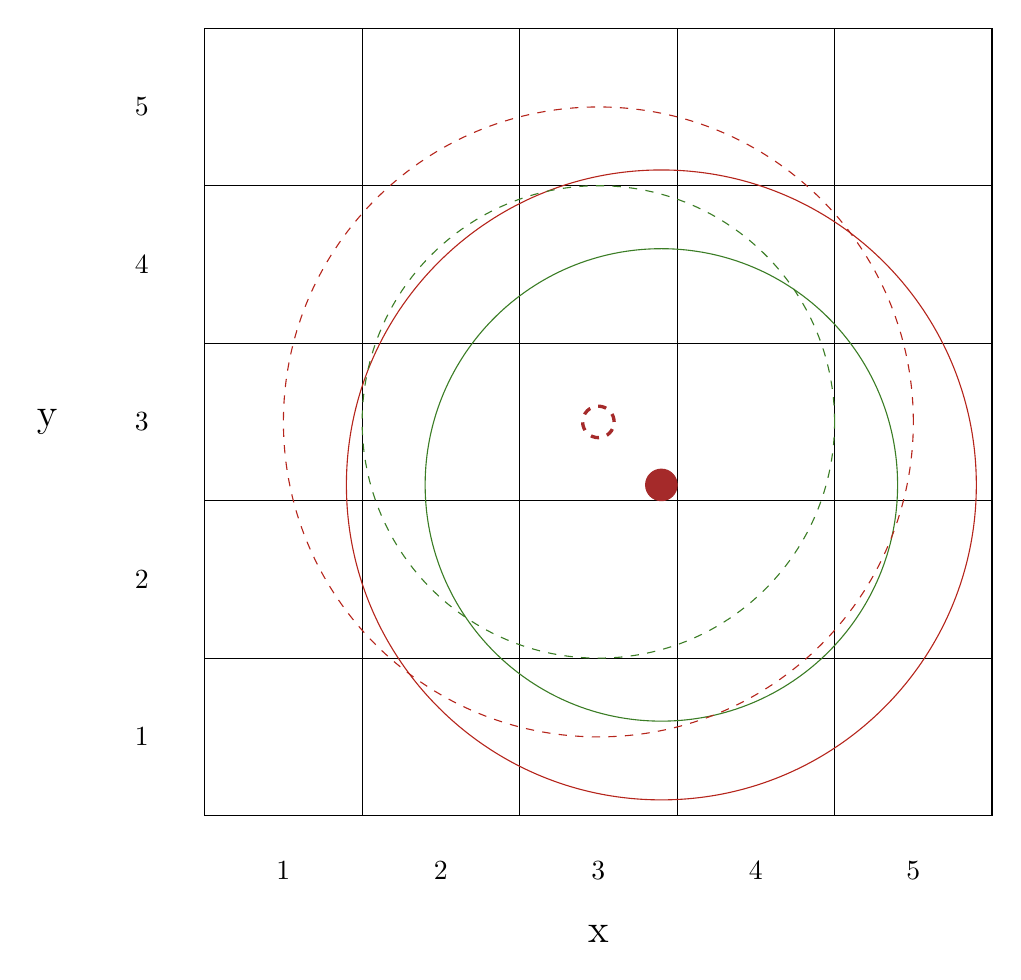
\begin{tikzpicture}[scale=2]
	% grid lines
	\draw (0, 0) grid (5, 5);

	% text coordinates
	\node at (-1, 2.5) {\Large{y}};
	\node at (2.5, -0.75) {\Large{x}};

	% coordinate values
	\foreach \i in {1,...,5} {
		\node at (\i-0.5, -0.35) {\i};
		\node at (-0.4, \i-0.5) {\i};
	}

	% filled unit
	\filldraw[Brown] (2.9, 2.1) circle(0.1);
	\draw[BrickRed] (2.9, 2.1) circle(2);
	\draw[OliveGreen] (2.9, 2.1) circle(1.5);

	% second dashed unit
	\draw[Brown,very thick,dashed] (2.5, 2.5) circle(0.1);
	\draw[BrickRed,dashed] (2.5, 2.5) circle(2);
	\draw[OliveGreen,dashed] (2.5, 2.5) circle(1.5);
\end{tikzpicture}
\caption{Example of using grid to minimize distance calculations. The brows dot (and dashed circle) represents the \textcolor{Brown}{unit}; green circle the \textcolor{OliveGreen}{include distance}; red circle the \textcolor{BrickRed}{exclude distance}. The dashed circles represents another unit, in the middle of a grid square, its include and exclude distances.}
\label{fig:player_squad_group_grid}
\end{figure}

Only units within two grid units are used when calculating the distance, this generats a 5x5 grid just as figure \ref{fig:player_squad_group_grid}. As can be seen in the figure units further away than two grid units can never be within the exclude distance. Units in the same grid or to the left, top, right, or bottom are almost always within the exclude distance, an exception can be seen in the figure where small portion of the upper left corner at (2,3) is outside the solid exclude circle; for simplicity all units are within these grid positions are automatically seen as within the exclude distance (even though exceptions might exist).

To make use of these calculation benefits, units in a squad are checked first (if they are further away than the exclude distance). A simplified pseudo-code expamle is listed below in listing \ref{lst:player_squad_rearrange_squads} where the high-level calculations are made and in listing \ref{lst:player_squad_add_close_units_to_squad} where calculations of which units to add to the squad—note that units are not excluded form the squad here, they are not excluded until they are added in another squad which happens at the end of \texttt{rearrangeSquads()}.

\begin{lstlisting}[label={lst:player_squad_rearrange_squads},caption={Pseudo-code of \texttt{rearrangeSquads()}.}]
// Iterate through all squads taking one unit each turn
do {
	foundUnit = false;
	while (moreUnitsToCheck() && !foundUnit) {
		if (unitSquad.isValid() && unitSquad != CHECKED) {
			currentUnit = unit;
			foundUnit = true;
		}
	}
	
	if (foundUnit) {
		setUnitAsChecked(currentUnit);
		setSquadAsChecked(unitSquad);
		
		addCloseUnitsToSquad(currentUnit, unitSquad->getId());
	}
} while (foundUnit);

// Create new squads for the rest of the units that either
// went outside the squad's bounds or never had a squad
while (moreUnitsToCheck()) {
	setUnitAsChecked(unit);
	newSquad = new PlayerSquad();
	setSquadAsChecked(newSquad);
	addCloseUnitsToSquad(unit, newSquad->getId());
}
\end{lstlisting}

\begin{lstlisting}[label={lst:player_squad_add_close_units_to_squad},caption={Pseudo-code of \texttt{addCloseUnitsToSquad()}}]
// Add all units that are in the same square or the
// bordering left, top, right, bottom square.
foreach (square in same, or border square) {
	foreach (not checked unit in this square) {
		if (same squads as paramUnit) {
			queuedUnits.push_back(unit);
			setUnitAsChecked(unit);
		} else if (withinIncludeDistance(unit, paramUnit) {
			queuedUnits.push_back(unit);
			setUnitAsChecked(unit);
		}
	}
}

// Recursively check queued units, this is done afterwards so
// that all fast calculations can be done first
while (!queuedUnits.empty()) {
	addCloseUnitsToSquad(queuedUnits.front(), squadId);
	queuedUnits.pop_front();
}

// Directly recursive, instead of queueing units it will directly
// call addCloseUnits... because those units could add close units
// that were within bordering squares that otherwise would be
// calculated here using distance calculations.
// Uses the full 5x5 square, except squares already checked
foreach (other square) {
	foreach (not checked unit in this square) {
		if (same squad as paramUnit) {
			if (isWithinExcludeDistance(unit, paramUnit) {
				setUnitAsChecked(unit);
				addCloseUnitsToSquad(unit, squadId);
			}
		} else if (isWithinIncludeDistance(unit, paramUnit) {
			setUnitAsChecked(unit);
			addCloseUnitsToSquad(unit, squadId);
		}
	}
}
\end{lstlisting}


\subsection{Grouped classifying tests}
The idea is a common class using the facade pattern to group both easy and complicated tests into one class to minimize the coupling between classes, reuse code, and have to have the code in one place if a tests was to change (instead of changing it in several places)—e.g. a simple test like \texttt{canFrontalAttack(units)} which returns true if the unit size is larger or equal to the minimum number of units BATS needs for a frontal attack, \texttt{\justify return units.size() >= FRONTAL\_ATTACK\_UNITS\_MIN;}. None of the classifying classes modifies any data, thus all functions are const.

All three classes (although an enemy classification was not implemented) were supposed to have a common interface to make it easier to use all three classes without having to learn three different interfaces. Due to lack of time and not being the most important aspect this feature was skipped in this version.

\paragraph{Self classification}
This classifier groups together common tests for BATS and might not be seen as a classifier by all. Many tests used by the \nameref{sec:commander} and \nameref{sec:defense_manager} uses the self classifier to easier calculate their goals and decrease their coupling. Below is a list and a brief description of what the test does, although most of the names should be self-exlanatory.

\begin{function_description}
	\item[\texttt{bool areExpansionsSaturated()}] Tests if there exists enough workers to saturate all mineral patches.
	\item[\texttt{bool canDrop()}] If BATS have enough units to create a drop.
	\item[\texttt{bool canFrontalAttack()}] If BATS have enough free units to create an attack. This is only used for when BATS want to create an attack, if the teammate orders an attack it is enough with one unit.
	\item[\texttt{int getActiveExpansionCount()}] Number of active expansions, i.e. expansions with more than \classificationExpansionExpansionMineralsLow.
	\item[\texttt{double getLastExpansionStartTime()}] How many game seconds ago the last expansion was started.
	\item[\texttt{bool hasDrop()}] Checks if BATS has a drop.
	\item[\texttt{bool isAnExpansionLowOnMinerals()}] Checks if an expansion has less than \classificationExpansionExpansionMineralsLow.
	\item[\texttt{bool isAttacking()}] Checks if we have an attack squads that is not retreating.
	\item[\texttt{bool isExpanding()}] Checks if BATS is either expanding or going to expand (expansions in build order).
	\item[\texttt{bool isHighOnGas()}] BATS has more than \classificationHighOnGas~gas.
	\item[\texttt{bool isHighOnMinerals()}] BATS has more than \classificationHighOnMinerals~minerals.
	\item[\texttt{bool isScouting()}] If BATS has a scout squad out.
	\item[\texttt{bool isUnderAttack()}] Checks if BATS is under attack, uses Defense Manager's isUnderAttack().
	\item[\texttt{bool isUpgradeSoonDone(affectedUnits)}] Checks if an upgrade, that will affect the specified units, completes within \classificationUpgradeSoonDone.
\end{function_description}

\paragraph{Teammate classification}
The teammate classification works just as the self classifier described above, but at the moment only has one function: \texttt{isExpanding()} which tests if the teammate constructs a new base structure (e.g. Command Center). As the squad functionality was implemented in \texttt{PlayerArmyManager}.